\question
(0,5 балла) Муравьи с планеты N известны своими разумными способностями и сложными социальными структурами. Они строят колонии из уникальных многоугольных ячеек, создавая впечатляющие архитектурные сооружения. Муравьи соединяют палочки с помощью специального раствора, образуя соединения только между концами палочек. В одной колонии муравьи использовали 58 палочек, каждая из которых была скреплена с другой на 30 разных местах. Сколько муравьев обитает в этой удивительной колонии, если в каждой ячейке проживает один муравей?

\begin{minipage}[h]{0.45\linewidth}
\center{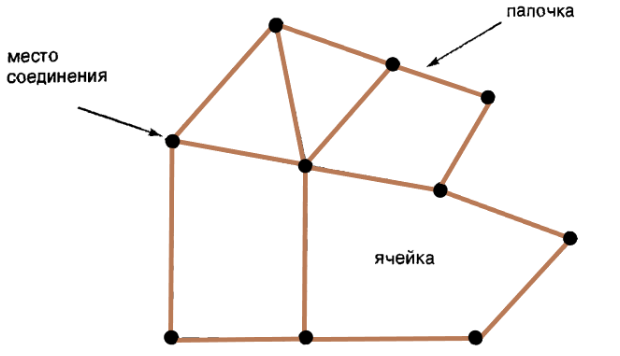
\includegraphics[width=0.7\textwidth]{pic/91.png} }
\end{minipage}

---------------

Автор -- Александр Лазарев, M3314
